%%%%%%%%%%%%%%%%%%%%%%%%%%%%%%%%%%%%%%%%%%%%%%%%%%%%%%%%%%%%%%%%%%%%%%%%%%%%%%%%%%%%%%%%%%%%%%%%%%%%
% ==================================================================================================
% --------------------------------------------------------------------------------------------------
\chapter{Experiment \& Results}
This section explores model validation. Performance of model components is characterized with respect to intermediate objectives, including graylevel standardization and regularization in toy scenarios. The segmentation performance of the full model is then presented under several cross validation frameworks, and compared to a similar algorithm.
%%%%%%%%%%%%%%%%%%%%%%%%%%%%%%%%%%%%%%%%%%%%%%%%%%%%%%%%%%%%%%%%%%%%%%%%%%%%%%%%%%%%%%%%%%%%%%%%%%%%
\section{Cross Validation Frameworks}\label{s:CVframeworks}
Supervised segmentation models require the capacity to model complex relationships between the input image(s) and output label images. When models with large capacity are trained on a dataset which does not represent the full gamut of potential input data, they risk \textit{overfitting}: acquiring a bias towards the training data \cite{Hawkins2004}. The main problem associated with overfitting is decreased performance on new data (\textsc{aka} generalization performance) \cite{Hawkins2004}. Popular techniques for characterizing this expected decrease include cross validation (CV) procedures. These involve splitting the $N$ available examples into training ($t$) and testing ($e$) subsets, where the training data are used to fit the model parameters, and the test data are used to approximate the expected generalization performance; the data splits are usually repeated, randomly or exhaustively, to ensure robust results \cite{Arlot2010}. The most popular CV frameworks include:
\begin{itemize}
  \item \textbf{LOO -- Leave-One-Out:} Withhold one example from the training set, and use it as the test case ($N_t$ = $N-1$; $N_e = 1$); repeat $N$ times.
  \\\textit{Benefit:} Close approximation of the expected generalization performance
  \\\textit{Drawback:} Expensive to compute -- $\mathcal{O}(N)$
  \item \textbf{KFCV -- K-Fold Cross Validation:} Withhold a random batch of $B = N/K$ examples from the training set, and use it as the test set ($N_t$ = $N-B$; $N_e = B$); repeat $K$ times (without replacement).
  \\\textit{Benefit:} Less expensive to compute -- $\mathcal{O}(N/K)$
  \\\textit{Drawback:} Worse approximation of the expected generalization performance
\end{itemize}
% ==================================================================================================
\subsection{Leave-One-Source-Out CV}
The choice of cross validation framework can have significant impacts on the reported model performance (see \cite{Arlot2010} for an in-depth review), and there is at least one assumption of the above methods which is not always valid: that examples are independent and identically distributed (iid). This is not true for data originating from multiple sources with different underlying distributions (e.g. MRI with different scan-parameter combinations) \cite{Geras2013}. In fact, \citeauthor{Geras2013} show that in multi-source problems where the expected use case involves data from entirely new sources, random KFCV (and therefore also LOO, as a special case of KFCV with $B=1$) significantly overestimates the generalization performance. This is because random training fold selection allows the model to perceive source-specific characteristics of the test examples, which cannot be repeated for truly new examples. In such scenarios, the authors propose the following:
\begin{itemize}
  \item \textbf{LOSO -- Leave-One-Source-Out\footnote{Authors' original name was ``Multi-Source Cross Validation''}:} Withhold all examples from source $s\in 1\dots S$ from the training set, and use these as the test set ($N_t$ = $N-N_s$; $N_e = N_s$); repeat $S$ times.
  \\\textit{Benefit:} Best approximation of the expected generalization performance in multi-source problems
  \\\textit{Drawback:} Still only an approximation
\end{itemize}
As noted in the introduction (cf. \S\ \ref{ss:priorlimits}), there has been surprisingly limited use of data from multiple sources for validation of WMH segmentation algorithms. Moreover, CV frameworks vary widely among papers, and to the best of this author's knowledge, no WMH algorithm has yet been validated using LOSO CV. This represents a significant caveat to reported performances, since MRI have many sources of variability (cf. \S\ \ref{ss:autochallenges}), including scanner manufacturer, field strength, sequence parameters, resolution, anatomical and disease variability. As the aim of this work is to develop a segmentation algorithm which will perform well on any given FLAIR MRI, the LOSO framework was initially developed without knowledge of the work by \citeauthor{Geras2013}. However, this paper happily corroborates the importance of LOSO CV to the current work. In this case, one data source is defined as a unique scanner-parameter combination.
% ==================================================================================================
\subsection{Competition Frameworks}\label{ss:competitions}
One notable exception to this trend in WMH algorithms have been segmentation competitions \cite{MSSEG2008,MSISBI2015,MSSEG2016,WMHSEG2017}. These generally provide both multi-source datasets and a robust validation framework.
Table \ref{tab:datacomp}
\begin{table}[h]
  \centering
  \caption{Summary of competition image databases.}
    \begin{tabu} to \textwidth {lccccc}
      \hline
      && \multicolumn{2}{c}{Training} & \multicolumn{2}{c}{Testing} \\
      Database     &       Ref.        & $I$ & $S$ & $I$ & $S$ \\ \hline
      WMH 2017     & \cite{WMHSEG2017} & 60  &  3  & 110 &  5  \\
      MS 2016      & \cite{MSSEG2016}  & 15  &  3  & 38  &  4  \\
      MS 2015 ISBI & \cite{MSISBI2015} & 21  &  1  & 61  &  1  \\
      MS 2008      & \cite{MSSEG2008}  & 20  &  2  & 32  &  2  \\ \hline
    \end{tabu}
  \label{tab:datacomp}
\end{table}

% ==================================================================================================
\subsection{Data}\label{ss:data}
For the reasons outlined above, it was important to collect a large and diverse database of FLAIR images for model validation. We use 129 FLAIR images from 10 different scanners. The number of images and scan parameters are summarized in Table \ref{tab:database}. With the exception of the MS 2008\footnotemark and In-House datasets, all of the data are freely available as part of the segmentation competitions. Since direct comparison of results on equal datasets is important for establishing state-of-the-art, we present results using only these freely available data (``Dataset A'') in addition to all .
\footnotetext{The manuals used with these data }
\begin{table}[t]
  \centering
  \caption{Summary of experimental image database.}
  {\setlength{\tabcolsep}{4pt}
    \begin{tabu} to \textwidth {crclX[c]X[c]X[c]cc}
      \hline
      Img  &                                          &                   &                    & TE   & TR    & TI   &         Voxel Size         & Manuals  \\
      (\#) &                                 Database &       Ref.        & Scanner            & (ms) & (ms)  & (ms) &            (mm)            &   (\#)   \\ \hline
       20  & WMH 2017 (1) {\color{c01}$\blacksquare$} & \cite{WMHSEG2017} & 3T Philips Achieva & 125  & 11000 & 2800 & $0.96\times0.96\times3.00$ & 1 \ss{a} \\
       20  & WMH 2017 (2) {\color{c02}$\blacksquare$} & \cite{WMHSEG2017} & 3T Siemens TrioTim & 82   & 9000  & 2500 & $1.00\times1.00\times3.00$ & 1 \ss{a} \\
       20  & WMH 2017 (3) {\color{c03}$\blacksquare$} & \cite{WMHSEG2017} & 3T GE Signa HDxt   & 126  & 8000  & 2340 & $0.98\times1.20\times3.00$ & 1 \ss{a} \\
       5   & MS 2016  (1) {\color{c04}$\blacksquare$} & \cite{MSSEG2016}  & 3T Philips Ingenia & 360  & 5400  & 1800 & $0.50\times1.10\times0.50$ & 7 \ss{b} \\
       5   & MS 2016  (2) {\color{c05}$\blacksquare$} & \cite{MSSEG2016}  & 1.5T Siemens Aera  & 336  & 5400  & 1800 & $1.04\times1.25\times1.04$ & 7 \ss{b} \\
       5   & MS 2016  (3) {\color{c06}$\blacksquare$} & \cite{MSSEG2016}  & 3T Siemens Verio   & 399  & 5000  & 1800 & $0.74\times0.70\times0.74$ & 7 \ss{b} \\
       21  & MS 2015 ISBI {\color{c07}$\blacksquare$} & \cite{MSISBI2015} & 3T Philips         & 68   & 11000 & 2800 & $0.43\times0.43\times3.00$ & 2 \ss{c} \\ \hline
       13  &     In-House {\color{c08}$\blacksquare$} &        ---        & 3T Philips Achieva & 125  & 9000  & 2800 & $1.00\times1.00\times1.00$ & 1 \ss{d} \\
       10  & MS 2008 CHB  {\color{c09}$\blacksquare$} & \cite{MSSEG2008}  & ---                & ---  & ---   & ---  & $0.50\times0.50\times0.50$ & 1 \ss{e} \\
       10  & MS 2008 UNC  {\color{c10}$\blacksquare$} & \cite{MSSEG2008}  & 3T Siemens Allegra & 125  & 9000  & 2800 & $0.50\times0.50\times0.50$ & 1 \ss{f} \\ \hline
    \end{tabu}}
  \tablepost{\ss{a}~Manuals were generated following the standards outlined in \cite{Caligiuri2015}, and were subsequently reviewed by a second rater, only WMH labels were included; \ss{b}~Manuals were fused using the LOP-STAPLE method \cite{Akhondi-Asl2014}; \ss{c}~Manuals were fused using logical `and'; \ss{d}~Manuals were generated in-house; \ss{e}~REVIEW; \ss{f}~REVIEW.}
  \label{tab:database}
\end{table}
%% ==================================================================================================
%\subsection{Baseline Model Performance}
%The remainder of this chapter explores model variants which hopefully yield performance improvements. For sake of comparison, we first present results from a minimal working algorithm. This version of the VLR model (``\texttt{base}'') is summarized in Table \ref{tab:hyperparams}.
%%%%%%%%%%%%%%%%%%%%%%%%%%%%%%%%%%%%%%%%%%%%%%%%%%%%%%%%%%%%%%%%%%%%%%%%%%%%%%%%%%%%%%%%%%%%%%%%%%%%
\section{Graylevel Standardization}



%%%%%%%%%%%%%%%%%%%%%%%%%%%%%%%%%%%%%%%%%%%%%%%%%%%%%%%%%%%%%%%%%%%%%%%%%%%%%%%%%%%%%%%%%%%%%%%%%%%%
\section{Regularization}


% ==================================================================================================
\subsection{Toy Model}\label{ss:toyreg}
In order to investigate the effect of different regularization strategies, a toy model is used. The model represents a single voxel during training, with synthetic observations. Regularizations are then chosen by hand to maintain desired characteristics in the fitted functions. 

\par
It is also possible to plot the MAP objective function $\J(\bb)$ in the 2D plane composed of $\bb = [\b^0,\b^1]$.
\begin{figure}
  \centering
  \begin{subfigure}{\plotwidth}\centering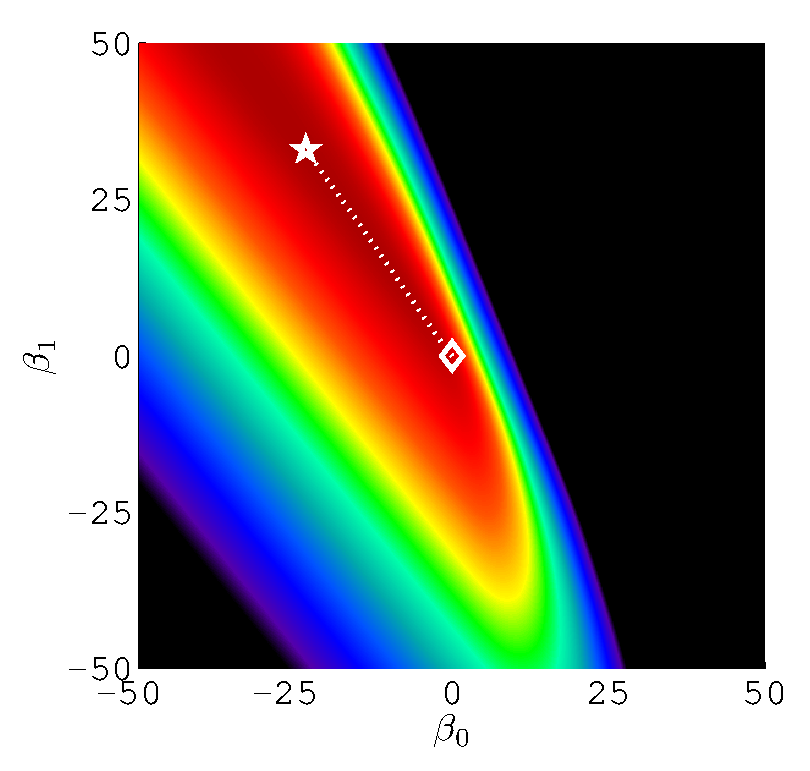
\includegraphics[height=7cm]{objective-surf}\caption{$\J(\bb)$ surface}\label{fig:obj-surf}\end{subfigure}
  \begin{subfigure}{\plotwidth}\centering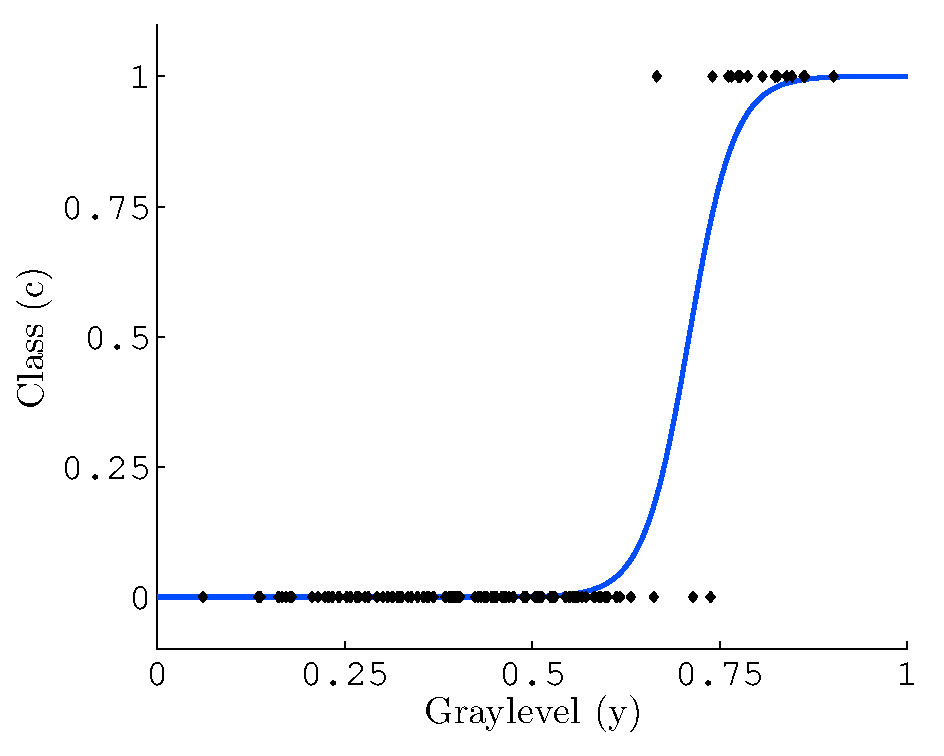
\includegraphics[height=7cm]{objective-LR}  \caption{Optimal model}\label{fig:obj-lr}\end{subfigure}
  \caption{MAP objective function in 2D; initialization (diamond), fitting (dotted), optimum (star).}
\end{figure}


%%%%%%%%%%%%%%%%%%%%%%%%%%%%%%%%%%%%%%%%%%%%%%%%%%%%%%%%%%%%%%%%%%%%%%%%%%%%%%%%%%%%%%%%%%%%%%%%%%%%
\section{Full Model}
% ==================================================================================================
\subsection{Convergence}
The rate of convergence in each voxel will be unique. During parallel fitting, it is prudent to stop training after a reasonable number of iterations, rather than wait for all voxels to achieve a certain stopping criterion, in case a few aberrant voxels do not converge. In order to determine this number, the model was fitted using [X] selection(s) of the training data, and the value of the MAP objective 
%__JK__ not sure how to chose this: see which are faster / slower?


% ==================================================================================================
\subsection{Parameter Images}\label{ss:paramimg}

For comparison with the LPA algorithm, the
\begin{figure}
  \centering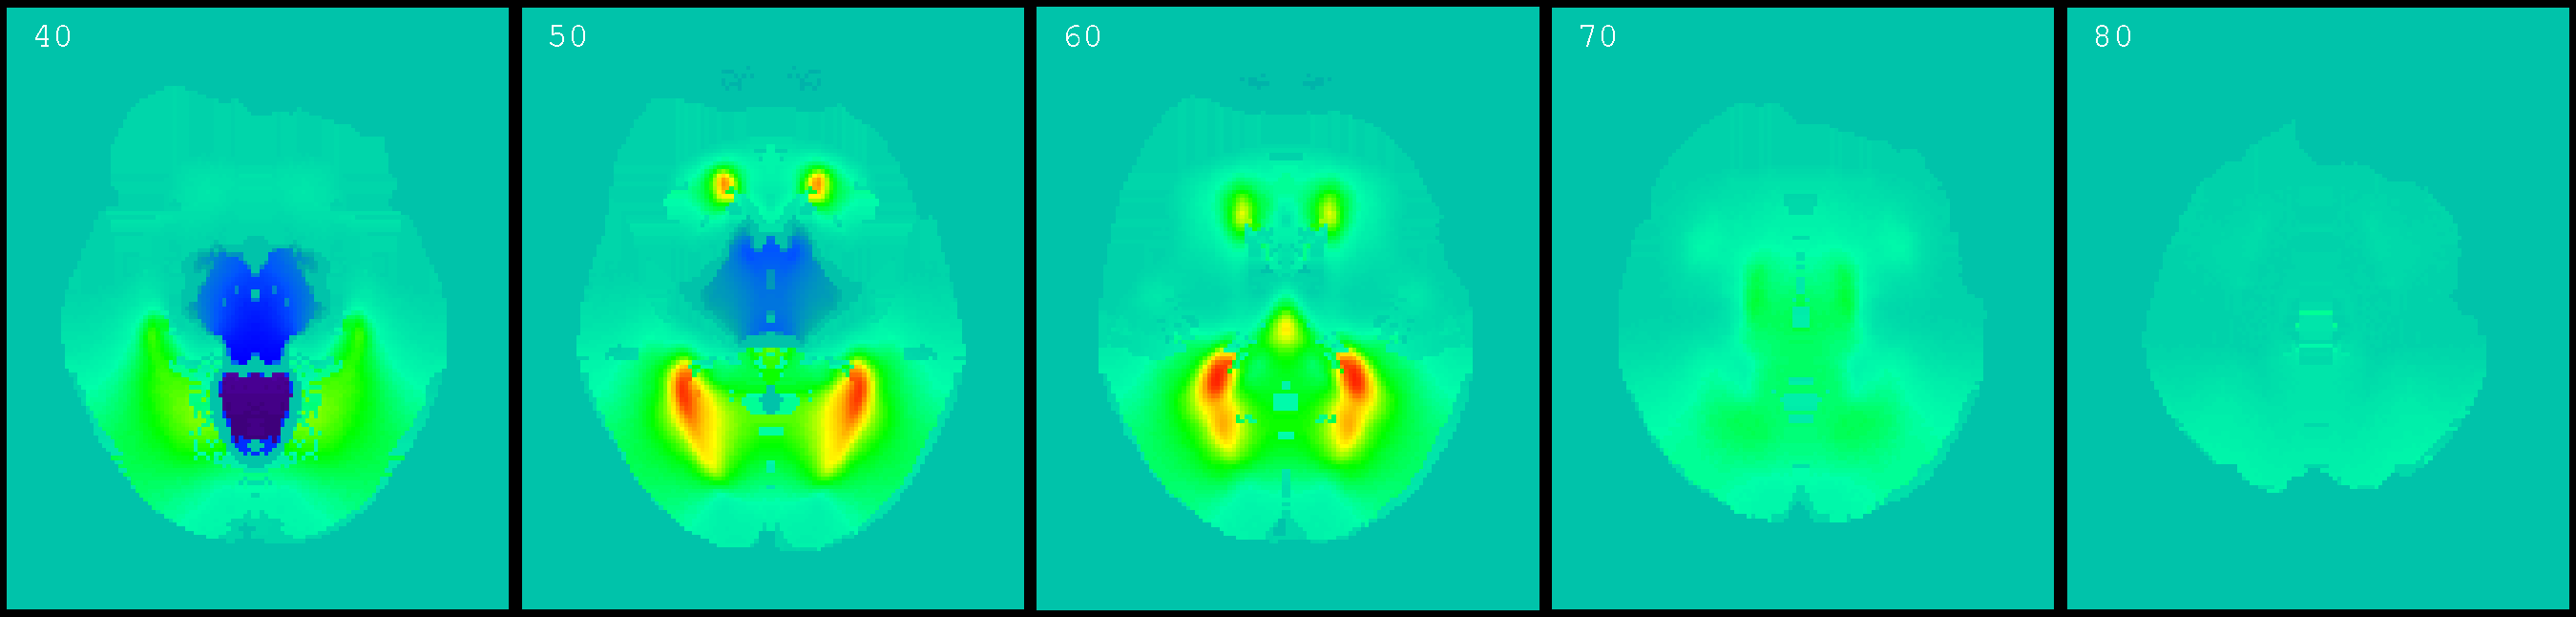
\includegraphics[height=\sliceheight]{beta-LPA.png} 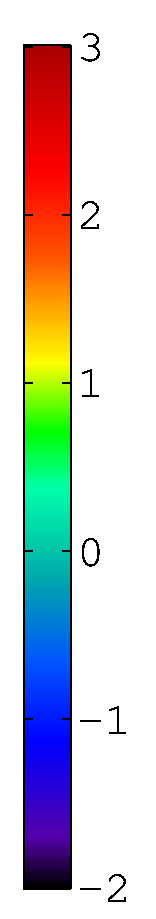
\includegraphics[height=\sliceheight]{cbar-NIH3-LPA}
  \caption{Spatial effect parameter image from the LPA toolbox after registration to MNI space.}
  \label{fig:B-lpa}
\end{figure}

% ==================================================================================================
\subsection{Quantitative Performance}
% --------------------------------------------------------------------------------------------------
\subsubsection{Regularization}
% ==================================================================================================
\subsection{Comparison with Another Method}
%%%%%%%%%%%%%%%%%%%%%%%%%%%%%%%%%%%%%%%%%%%%%%%%%%%%%%%%%%%%%%%%%%%%%%%%%%%%%%%%%%%%%%%%%%%%%%%%%%%%
\section{Discussion}
%To discuss:
%\begin{itemize}
%  \item central tendency in lesion load: due to histogram equalization. Solution: iteration
%\end{itemize}
% --------------------------------------------------------------------------------------------------
% ==================================================================================================
%%%%%%%%%%%%%%%%%%%%%%%%%%%%%%%%%%%%%%%%%%%%%%%%%%%%%%%%%%%%%%%%%%%%%%%%%%%%%%%%%%%%%%%%%%%%%%%%%%%%



%\newcommand{\di}{\mathrm{x}}
%\newcommand{\Di}{\mathrm{X}}
%\newcommand{\bDi}{\bm{\Di}}
%Consider a database composed of data from $S$ sources, $\bDi = \{\Di_1,\dots,\Di_S\}$, where $N_s$ is the number of examples from the $s$\ss{th} source, and $\Di_s = \{\di_1,\dots,\di_{\textsc{n}_s}\}$, so the total number of examples is $N_{\di} = \sum_{s}N_s$ ($\di$: inputs and outputs). Let $\bDi_r \subset\bDi$ be the training set, and $\bDi_e \subset \bDi$ be the test set. If $k$ is a CV repetition index, and then 
%
%The following CV frameworks can be defined:
%\begin{itemize}
%  \item \textbf{LOO -- Leave One Out:} $\bDi_r = \di_k$, $\bDi_e = \bDi\cup!\di_k$
%  \item \textbf{KFCV -- K-Fold Cross Validation:} 
%  \item \textbf{OSAAT -- One Source At A Time:}
%  \item \textbf{LOSO -- Leave One Source Out:} $\bDi_r = \Di_k$
%\end{itemize}
%Finally,  ... (cf. Training / Validation / Test Sets in \cite{Ripley1995})